\chapter{Méthodes}
	\section{Heuristiques constructives}
		Nous proposons deux heuristiques d'insertion. La première est pilotée par l'utilisateur et la seconde est autonome.

		Ces deux heuristiques servent à construire des solutions réalisables. L'optimalité de ces solutions n'est pas garantie et n'est pas un objectif. En effet, une heuristique est une étape de résolution qui vise seulement à produire une solution viable sur laquelle on pourra appliquer des modifications de manière itérative jusqu'à l'obtention d'un résultat répondant aux critères de qualité que l'on aura fixés.

		Il est très souvent plus facile d'améliorer un système dont on sait qu'il fonctionne que de chercher à rendre efficace un système défectueux.
		\subsection{Interception selon une séquence}
		\label{sub:heuristic_sequence}
			Dans cette heuristique, l'utilisateur fournit une séquence de mobiles à intercepter dans l'ordre de la lecture de cette séquence. L'heuristique est alors chargée pour chaque mobile de cette séquence de déterminer l'intercepteur capable de l'atteindre dans les meilleurs délais. On garantit alors la propriété suivante pour chaque tournée $r$:
			\[
				\forall i, j \qtext{t.q.}  i<j, \qtext{on a} \text{pos}(r_i) < \text{pos}(r_j)
			\]
			avec $r_k$ le mobile intercepté en $k$\ieme{} position dans la tournée $r$, et pos($r_k$) la fonction permettant d'obtenir la position du mobile $r_k$ dans la séquence imposée par l'utilisateur.

			La figure~\ref{fig:heuristic_sequence_demo} présente un exemple de solution réalisable.

			\begin{figure}[h!]
			\centering
			Séquence donnée: $\{4, 2, 3, 0, 1\}$

			\begin{tikzpicture}[schema]
				\begin{scope}[start chain=trunk]
	\node[interceptor, on chain, label=left:$I_0$] {};
	\node[mobile, on chain, join, label=above:$M_4$] {};
	\node[mobile, on chain, join, label=above:$M_0$] {};
	\node[interceptor, on chain, join] {};
\end{scope}
\begin{scope}[start chain=trunk,yshift=-1.25cm]
	\node[interceptor, on chain, label=left:$I_1$] {};
	\node[mobile, on chain, join, label=above:$M_2$] {};
	\node[mobile, on chain, join, label=above:$M_3$] {};
	\node[mobile, on chain, join, label=above:$M_1$] {};
	\node[interceptor, on chain, join] {};
\end{scope}

			\end{tikzpicture}
			\caption{Exemple de solution réalisable pour l'heuristique ``Séquence''}
			\label{fig:heuristic_sequence_demo}
			\end{figure}

		\subsection{Interception au plus tôt}
		\label{sub:heuristic_fastest}
			Dans cette heuristique, le calcul de chaque interception est piloté par le temps. L'heuristique calcule pour chaque insertion les meilleurs candidats (mobile et tournée). Il s'agit donc de déterminer quel est le mobile qui pourra être inseré dans la tournée réalisée par l'intercepteur capable de le rejoindre au plus tôt. Il s'agit d'une méthode plus gourmande en ressources, mais qui permet d'obtenir des résultats généralement de meilleure qualité que l'insertion par séquence.

			Afin d'optimiser les performances, nous avons développé une politique de \gls{cache} permettant de conserver une matrice des durées nécessaires pour atteindre chaque mobile à partir de chaque intercepteur. Ainsi, lorsqu'un mobile est intercepté, seules les durées relatives à l'intercepteur candidat sont faussées et doivent être recalculées, les durées nécessaires aux autres intercepteurs pour atteindre les autres mobiles restent identiques. Nous décrivons plus en détail ce mécanisme dans l'annexe~\ref{app:cache}.

			Toutefois, cette heuristique doit être utilisée avec parcimonie en raison de son coût de calcul, mais aussi car elle n'est pas paramétrable et n'offre donc pas de capacités d'extension de ses possibilités, notamment le fait d'ignorer des mobiles ou de prioriser l'interception d'un mobile par rapport à un autre sur une décision arbitraire.

			\begin{figure}[h!]
				\begin{subfigure}[t]{.5\linewidth}
					\centering
					\caption{Au plus tôt}
					\label{subfig:fastest_demo}
					\begin{tikzpicture}[scale=.5,baseline]
						\draw[grided,step=1.0,thin] (-3,-2) grid (12,12);
\draw[color=Gray] (-3,0) -- coordinate (x axis mid) (12,0);
\draw[color=Gray] (0,-2) -- coordinate (x axis mid) (0,12);
\foreach \x in {-3,...,12}
\draw[color=Gray] (\x,1pt) -- (\x,-3pt) node[anchor=north] {\x};
\foreach \y in {-2,...,12}
\draw[color=Gray] (1pt,\y) -- (-3pt,\y) node[anchor=east] {\y};
\node[interceptor] (D0) at (0,0) {\interceptor};
\node (I0) at (D0) {};
\node[interceptor] at ($ (I0) + (315:0.4) $) {$I_0$};
\node[interceptor] (D1) at (12,12) {\interceptor};
\node (I1) at (D1) {};
\node[interceptor] at ($ (I1) + (315:0.4) $) {$I_1$};
\node[mobile,anchor=center] (M0) at (1,2) {\mobile};
\node[mobile] at (M0.south east) {$M_{0}$};
\draw[speed] (M0.center) -- ($ (M0.center) + (-1,0) $);
\node[mobile,anchor=center] (M1) at (4,1) {\mobile};
\node[mobile] at (M1.south east) {$M_{1}$};
\draw[speed] (M1.center) -- ($ (M1.center) + (0.5,0.5) $);
\node[mobile,anchor=center] (M2) at (0,3) {\mobile};
\node[mobile] at (M2.south east) {$M_{2}$};
\draw[speed] (M2.center) -- ($ (M2.center) + (0,-1) $);
\node[mobile,anchor=center] (M3) at (2,5) {\mobile};
\node[mobile] at (M3.south east) {$M_{3}$};
\draw[speed] (M3.center) -- ($ (M3.center) + (1,0.3) $);
\node[mobile,anchor=center] (M4) at (-1,-2) {\mobile};
\node[mobile] at (M4.south east) {$M_{4}$};
\draw[speed] (M4.center) -- ($ (M4.center) + (-0.5,0.5) $);
\draw[direction] (M0.center) -- (2.22045e-16,2);
\draw[interceptor] (0,0) -- (2.22045e-16,2);
\node[interceptor] at (2.22045e-16,2) {\mobile};
\draw[direction] (M2.center) -- (0,2);
\draw[interceptor] (2.22045e-16,2) -- (0,2);
\node[interceptor] at (0,2) {\mobile};
\draw[direction] (M4.center) -- (-2.38482,-0.615179);
\draw[interceptor] (0,2) -- (-2.38482,-0.615179);
\node[interceptor] at (-2.38482,-0.615179) {\mobile};
\draw[interceptor](-2.38482,-0.615179) node[anchor=north west] {$t_{0}=2.76964$};
\draw[direction] (M3.center) -- (6.11793,6.23538);
\draw[interceptor] (12,12) -- (6.11793,6.23538);
\node[interceptor] at (6.11793,6.23538) {\mobile};
\draw[direction] (M1.center) -- (6.70783,3.70783);
\draw[interceptor] (6.11793,6.23538) -- (6.70783,3.70783);
\node[interceptor] at (6.70783,3.70783) {\mobile};
\draw[interceptor](6.70783,3.70783) node[anchor=north east] {$t_{1}=5.41567$};

					\end{tikzpicture}
				\end{subfigure}
				\hfill
				\begin{subfigure}[t]{.5\linewidth}
					\centering
					\caption{Par séquence}
					\label{subfig:_sequence_demo}
					\begin{tikzpicture}[scale=.5,baseline]
						\tikzset{interceptor/.style = {thick, color=OrangeRed}}
						\draw[grided,step=1.0,thin] (-7,-7) grid (12,12);
\draw[color=Gray] (-7,0) -- coordinate (x axis mid) (12,0);
\draw[color=Gray] (0,-7) -- coordinate (x axis mid) (0,12);
\foreach \x in {-7,...,12}
\draw[color=Gray] (\x,1pt) -- (\x,-3pt) node[anchor=north] {\x};
\foreach \y in {-7,...,12}
\draw[color=Gray] (1pt,\y) -- (-3pt,\y) node[anchor=east] {\y};
\node[interceptor] (D0) at (0,0) {\interceptor};
\node (I0) at (D0) {};
\node[interceptor] at ($ (I0) + (315:0.4) $) {$I_0$};
\node[interceptor] (D1) at (12,12) {\interceptor};
\node (I1) at (D1) {};
\node[interceptor] at ($ (I1) + (315:0.4) $) {$I_1$};
\node[mobile,anchor=center] (M0) at (1,2) {\mobile};
\node[mobile] at (M0.south east) {$M_{0}$};
\draw[speed] (M0.center) -- ($ (M0.center) + (-1,0) $);
\node[mobile,anchor=center] (M1) at (4,1) {\mobile};
\node[mobile] at (M1.south east) {$M_{1}$};
\draw[speed] (M1.center) -- ($ (M1.center) + (0.5,0.5) $);
\node[mobile,anchor=center] (M2) at (0,3) {\mobile};
\node[mobile] at (M2.south east) {$M_{2}$};
\draw[speed] (M2.center) -- ($ (M2.center) + (0,-1) $);
\node[mobile,anchor=center] (M3) at (2,5) {\mobile};
\node[mobile] at (M3.south east) {$M_{3}$};
\draw[speed] (M3.center) -- ($ (M3.center) + (1,0.3) $);
\node[mobile,anchor=center] (M4) at (-1,-2) {\mobile};
\node[mobile] at (M4.south east) {$M_{4}$};
\draw[speed] (M4.center) -- ($ (M4.center) + (-0.5,0.5) $);
\draw[direction] (M0.center) -- (2.22045e-16,2);
\draw[interceptor] (0,0) -- (2.22045e-16,2);
\node[interceptor] at (2.22045e-16,2) {\mobile};
\draw[direction] (M1.center) -- (6.02906,3.02906);
\draw[interceptor] (2.22045e-16,2) -- (6.02906,3.02906);
\node[interceptor] at (6.02906,3.02906) {\mobile};
\draw[direction] (M2.center) -- (0,-6.84105);
\draw[interceptor] (6.02906,3.02906) -- (0,-6.84105);
\node[interceptor] at (0,-6.84105) {\mobile};
\draw[interceptor](0,-6.84105) node[anchor=south east] {$t_{0}=9.84105$};
\draw[direction] (M3.center) -- (6.11793,6.23538);
\draw[interceptor] (12,12) -- (6.11793,6.23538);
\node[interceptor] at (6.11793,6.23538) {\mobile};
\draw[direction] (M4.center) -- (-6.23744,3.23744);
\draw[interceptor] (6.11793,6.23538) -- (-6.23744,3.23744);
\node[interceptor] at (-6.23744,3.23744) {\mobile};
\draw[interceptor](-6.23744,3.23744) node[anchor=north west] {$t_{1}=10.4749$};

					\end{tikzpicture}
				\end{subfigure}
				\caption{Application des heuristiques d'insertion}
				\label{fig:heuristics_demo}
			\end{figure}


	\section{Recherche Locale et optimisation bi-critères}
		La recherche locale vise à améliorer une solution en réalisant une succession de mutations simples. En effet, lorsque l'heuristique d'insertion se termine, deux cas se présentent:
		\begin{itemize}
			\item Tous les mobiles ont été interceptés,
			\item Il reste un ou plusieurs mobiles non-interceptés.
		\end{itemize}

		Dans le premier cas, le moyen le plus simple pour gagner du temps consiste à retirer un mobile, c'est le mouvement présenté dans la section \ref{subs:move_extract}. Dans le second cas, on peut essayer d'insérer les mobiles restants dans une tournée (section \ref{subs:move_insert}).

		Il est également possible de combiner ces deux mouvements élémentaires pour former quel\-ques mouvements plus complexes, par exemple enlever un mobile pour le déplacer dans une autre tournée, ou ailleurs dans la même tournée. Nous présentons donc plusieurs mouvements que nous jugeons pertinents dans les sections suivantes.

		Il est cependant nécessaire de veiller à ce que les mouvements ainsi décrits soient appliqués stratégiquement, car l'objectif est d'améliorer la solution et non de la détériorer. Il convient donc de fixer les limites d'une détérioration que l'on jugera acceptable. L'intérêt d'autoriser une légère détérioration est que celle-ci ne peut être que temporaire, pour permettre la validation d'un autre mouvement qui laissera ensuite envisager une amélioration plus forte.

		Les objectifs de qualité pour une solution sont le nombre de mobiles interceptés et la date de fin de la tournée la plus longue (en termes de durée). C'est la raison pour laquelle nous avons défini des politiques d'amélioration visant à atteindre ces objectifs qui sont mutuellement contradictoires, tout en garantissant que les limites de détérioration ne soient pas dépassées. Ces politiques définissent quelle est la solution à choisir et valident (ou invalident) des propositions de modification. Elles sont décrites dans les sections \ref{subs:first_available_policy} et \ref{subs:best_available_policy}.

		\subsection{Mouvements améliorants}

		\subsubsection{Mouvement d'extraction}
			Le mouvement d'extraction permet de retirer un mobile dans une tournée afin d'améliorer le pire temps d'interception. Pour cela, seule la suppression d'un mobile dans la tournée la plus longue en temps sera validée, car une extraction dans les autres tournées n'apporterait pas d'amélioration globale à la solution. Afin que ce mouvement ne vide pas successivement les tournées jusqu'à aboutir à une solution où aucun mobile n'est intercepté (solution triviale pour la minimisation du temps), une politique a été ajoutée pour considérer le problème avec le critère de temps, mais aussi celui du nombre de mobiles. Un minimum est donc fixé pour ne pas aller en-dessous d'un certain seuil.
			
			
			L'algorithme de principe est le suivant :
			\begin{code}
				\begin{algo}[informal]
					\ALGO{Principe d'extraction d'un mobile dans une tournée}
					\BEGIN
						\STATE{Amélioration ← Faux}
						\STATE{Récupérer la pire tournée t en temps}
						\FORGEN{tous les mobiles m dans la tournée t faire}
							\STATE{Calculer le temps d'interception de la tournée sans le mobile m}
							\IF{le temps d'interception est fini et que la politique est respectée}
								\STATE{Amélioration ← Vrai}
							\ENDIF
						\ENDFORGEN
						\RETURN{Amélioration}
					\END
				\end{algo}
				\captionof{listing}{Algorithme de principe -- Extraction d'un mobile dans une tournée}
			\end{code}
			
			\label{subs:move_extract}
			\begin{figure}[h!]
			\centering
			\begin{tikzpicture}[schema]
				\begin{scope}[start chain, x=0,y=0]
	\node[interceptor, on chain] {};
	\node[mobile, on chain, join] {};
	\node[mobile, on chain, join] (B) {};
	\node[mobile, on chain, join,red] (E) {};
	\node[mobile, on chain, join] (A) {};
	\node[interceptor, on chain, join] {};
\end{scope}
\draw[correction,dotted] (B) to[bend right] (A);
\draw[correction] (E) -- ($ (E) + (0,1) $);
\node[right= .5 of B,cross] {$\times$};
\node[right= .5 of E,cross] {$\times$};

			\end{tikzpicture}
			\caption{Schéma d'extraction d'un mobile hors d'une tournée}
			\label{fig:move_extract}
			\end{figure}

		\subsubsection{Mouvement d'insertion}
			Le mouvement d'insertion permet d'ajouter un mobile à une tournée. Il est donc forcément améliorant en terme de mobiles, mais il peut alors impacter le temps maximum d'interception. Ce mouvement sera donc validé uniquement s'il ne l'augmente pas.
			
			L'algorithme de principe est le suivant :
			\begin{code}
				\begin{algo}[informal]
					\ALGO{Principe d'insertion d'un mobile dans une tournée}
					\BEGIN
						\FORGEN{tous les mobiles non interceptés m}
							\FORGEN{toutes les tournées t}
								\FORGEN{toutes les positions p}
									\STATE{Calculer le temps d'interception en insérant m dans t à la position p}
									\IF{l'insertion est possible (le temps est fini)}
										\STATE{Comparer le résultat obtenu avec le temps initial (avec arrêt de la recherche selon les politiques)}
									\ENDIF
								\ENDFORGEN
							\ENDFORGEN
						\ENDFORGEN
						\RETURN{vrai s'il y a eu amélioration, faux sinon}
					\END
				\end{algo}
				\captionof{listing}{Algorithme de principe -- Insertion d'un mobile dans une tournée}
			\end{code}
					
		
			\label{subs:move_insert}
			\begin{figure}[h!]
			\centering
			\begin{tikzpicture}[schema]
				\begin{scope}[start chain,x=0,y=0]
	\node[interceptor, on chain] {};
	\node[mobile, on chain, join] {};
	\node[mobile, on chain, join] (B) {};
	\node[mobile, on chain, join] (A) {};
	\node[mobile, on chain, join] {};
	\node[interceptor, on chain, join] {};
\end{scope}
\node[right= .5 of B,cross] (X) {$\times$};
\node[mobile, below= .5 of X,red] (I) {};
\draw[correction,dotted] (B) -- (I);
\draw[correction,dotted] (I) -- (A);

			\end{tikzpicture}
			\caption{Schéma d'insertion d'un mobile dans une tournée}
			\label{fig:move_insert}
			\end{figure}

		\subsubsection{Mouvement de substitution (ou remplacement)}
				Le mouvement de substitution permet d'insérer un mobile à la place d'un autre mobile dans une tournée. Il s'agit donc d'un mouvement de suppression suivi d'un mouvement d'insertion. Comme le nombre de mobile ne change pas, seul le gain de temps est considéré pour valider ou non l'opération.
				
				L'algorithme de principe est le suivant :
				\begin{code}
					\begin{algo}[informal]
						\ALGO{Principe du remplacement dans une tournée}
						\BEGIN
							\FORGEN{tous les mobiles non interceptés m}
								\FORGEN{toutes les tournées t}
									\FORGEN{tous les mobiles m' dans t}
										\STATE{Calculer le temps d'interception en remplaçant m' par m dans t}
										\STATE{Comparer le résultat obtenu avec le temps initial (avec arrêt de la recherche selon les politiques)}
									\ENDFORGEN
								\ENDFORGEN
							\ENDFORGEN
							\RETURN{vrai s'il y a eu amélioration, faux sinon}
						\END
					\end{algo}
				\captionof{listing}{Algorithme de principe -- Remplacement d'un mobile dans une tournée}
			\end{code}
			
			\begin{figure}[h!]
			\centering
			\begin{tikzpicture}[schema]
				\begin{scope}[start chain]
	\node[interceptor, on chain] {};
	\node[mobile, on chain, join] {};
	\node[mobile, on chain, join] (B) {};
	\node[mobile, on chain, join,red] (R) {};
	\node[mobile, on chain, join] (A){};
	\node[interceptor, on chain, join] {};
\end{scope}
\node[right= .5 of B,cross] (X) {$\times$};
\node[right= .5 of R,cross] {$\times$};
\node[mobile, below= .5 of R,red] (I) {};
\draw[correction,dotted] (B) -- (I);
\draw[correction,dotted] (I) -- (A);
\draw[correction] (R) -- ($ (R) + (0,1) $);

			\end{tikzpicture}
			\caption{Schéma de substitution d'un mobile dans une tournée}
			\label{fig:move_replace}
			\end{figure}

		\subsubsection{Mouvements de déplacement}
			Le mouvement de déplacement d'un mobile dans une tournée consiste à changer de position l'un des mobiles au sein de la même tournée. L'objectif est de trouver une meilleure organisation de la tournée et donc d'obtenir un gain de temps sur la date d'interception finale.

			L'algorithme de principe est le suivant:
			\begin{code}
				\begin{algo}[informal]
					\ALGO{Principe du déplacement dans une tournée}
					\BEGIN
						\FORGEN{toutes les tournées t}
							\FORGEN{toutes les positions p possibles dans t}
								\FORGEN{tous les mobiles m}
									\IF{le déplacement existe}
										\STATE{Calculer le nouveau temps d'interception de t avec le déplacement de m dans la tournée.}
										\STATE{Comparer le résultat obtenu avec le temps initial (avec arrêt de la recherche selon les politiques)}
									\ENDIF
								\ENDFORGEN
							\ENDFORGEN
						\ENDFORGEN
						\RETURN{vrai s'il y a eu amélioration, faux sinon}
					\END
				\end{algo}
				\captionof{listing}{Algorithme de principe -- Déplacement au sein d'une tournée}
			\end{code}


			Le mouvement de déplacement d'un mobile dans une autre tournée consiste à supprimer un mobile de sa tournée pour l'insérer dans une seconde tournée.

			L'algorithme de principe est le suivant :
			\begin{code}
				\begin{algo}[informal]
					\ALGO{Principe du déplacement dans deux tournées}
					\BEGIN
						\FORGEN{toutes les tournées t1}
							\FORGEN{tous les mobiles m dans t1}
								\FORGEN{toutes les tournées t2}
									\FORGEN{toutes les positions dans t2}
										\STATE{Calculer le nouveau temps d'interception de t2 avec l'insertion de m à la position p}
										\STATE{Comparer le résultat obtenu avec le temps inital (avec arrêt de la recherche selon les politiques)}
									\ENDFORGEN
								\ENDFORGEN
							\ENDFORGEN
						\ENDFORGEN
						\RETURN{vrai s'il y a eu amélioration, faux sinon}
					\END
				\end{algo}
				\captionof{listing}{Algorithme de principe -- Déplacement d'un mobile au sein d'une autre tournée}
			\end{code}

			\begin{figure}[h!]
			\begin{subfigure}[b]{.54\linewidth}
				\centering
				\begin{tikzpicture}[schema]
					\begin{scope}[start chain]
	\node[interceptor, on chain] {};
	\node[mobile, on chain, join] (B) {};
	\node[mobile, on chain, join,red] (M) {};
	\node[mobile, on chain, join] (A) {};
	\node[mobile, on chain, join] (I) {};
	\node[mobile, on chain, join] (IA) {};
	\node[interceptor, on chain, join] {};
\end{scope}
\draw[correction,dotted] (B) to[bend right] node[stepnode] {1} (A);
\draw[correction,dotted] (I) to[bend right] node[stepnode] {2} (M);
\draw[correction,dotted] (M) to[bend left, out=60, in=120] node[stepnode] {3} (IA);
\node[right= .5 of M,cross] {$\times$};
\node[right= .5 of B,cross] {$\times$};
\node[right= .5 of I,cross] (X) {$\times$};
\draw[correction] (M) to[bend right] (X);

				\end{tikzpicture}
				\subcaption{Au sein d'une même tournée}
				\label{subfig:move_move1route}
			\end{subfigure}
			\hfill
			\begin{subfigure}[b]{.45\linewidth}
				\centering
				\begin{tikzpicture}[schema]
					\begin{scope}[start chain]
	\node[interceptor, on chain] {};
	\node[mobile, on chain, join] (B) {};
	\node[mobile, on chain, join,red] (M) {};
	\node[mobile, on chain, join] (A) {};
	\node[interceptor, on chain, join] {};
\end{scope}
\begin{scope}[start chain, yshift=-1.25cm]
	\node[interceptor, on chain] {};
	\node[mobile, on chain, join] {};
	\node[mobile, on chain, join] (I) {};
	\node[mobile, on chain, join] (IA) {};
	\node[mobile, on chain, join] {};
	\node[interceptor, on chain, join] {};
\end{scope}
\draw[correction,dotted] (I) -- node[stepnode] {1} (M);
\draw[correction,dotted] (M) -- node[stepnode] {2} (IA);
\draw[correction,dotted] (B) to[bend left] node[stepnode] {3} (A);
\node[right= .5 of M,cross] {$\times$};
\node[right= .5 of B,cross] {$\times$};
\node[right= .5 of I,cross] (X) {$\times$};
\draw[correction] (M) -- (X);


				\end{tikzpicture}
				\subcaption{Entre deux tournées}
				\label{subfig:move_move2routes}
			\end{subfigure}
			\caption{Schéma de déplacement d'un mobile}
			\label{fig:move_move}
			\end{figure}

		\subsubsection{Mouvements d'interversion (ou swap)}
			Le mouvement d'interversion ou swap consiste à échanger deux mobiles déjà présents dans une tournée. Il existe deux variantes de ce mouvement : lorsque les deux mobiles appartiennent à la même tournée ou lorsque les tournées sont différentes. Étant donné que ce mouvement ne peut pas diminuer le nombre de mobiles traités, le critère d'amélioration porte uniquement sur la réduction du temps final de la ou l'une des tournées considérées.

			L'algorithme de principe pour l'interversion dans une même tournée est le suivant:
			\begin{code}
				\begin{algo}[informal]
					\ALGO{Principe de l'interversion dans une tournée}
					\BEGIN
						\FORGEN{toutes les tournées t}
							\FORGEN{tous les mobiles m1 dans t}
								\FORGEN{tous les mobiles m2 après m1 dans t}
									\STATE{Calculer le nouveau temps d'interception de t avec m2 à la place de m1}
									\STATE{Comparer le résultat obtenu avec le temps initial (avec arrêt de la recherche selon les politiques)}
								\ENDFORGEN
							\ENDFORGEN
						\ENDFORGEN
						\RETURN{vrai s'il y a eu amélioration, faux sinon}
					\END
				\end{algo}
				\captionof{listing}{Algorithme de principe -- Interversion au sein d'une même tournée}
			\end{code}

			L'algorithme de principe pour l'interversion avec deux tournées est le suivant :
			\begin{code}
				\begin{algo}[informal]
					\ALGO{Principe de l'interversion entre deux tournées}
					\BEGIN
						\FORGEN{toutes les tournées t1 sauf la dernière}
							\FORGEN{toutes les tournées t2 après t1}
								\FORGEN{tous les mobiles m1 dans t1}
									\FORGEN{tous les mobiles m2 dans t2}
										\STATE{Calculer le nouveau temps d'interception de t1 avec m2 à la place de m1}
										\STATE{Calculer le nouveau temps d'interception de t2 avec m1 à la place de m2}
										\STATE{Comparer les résultats obtenus avec les temps initiaux (avec arrêt de la recherche selon les politiques)}
									\ENDFORGEN
								\ENDFORGEN
							\ENDFORGEN
						\ENDFORGEN
						\RETURN{vrai s'il y a eu amélioration, faux sinon}
					\END
				\end{algo}
				\captionof{listing}{Algorithme de principe -- Interversion entre deux tournées}
			\end{code}


			\begin{figure}[h!]
			\begin{subfigure}[b]{.54\linewidth}
				\centering
				\begin{tikzpicture}[schema]
					\begin{scope}[start chain]
	\node[interceptor, on chain] (B1) {};
	\node[mobile, on chain, join,red] (S1) {};
	\node[mobile, on chain, join] (A1) {};
	\node[mobile, on chain, join] (B2) {};
	\node[mobile, on chain, join,red] (S2) {};
	\node[mobile, on chain, join] (A2) {};
	\node[interceptor, on chain, join] {};
\end{scope}
\draw[correction,dotted] (B1) to[bend right] node[stepnode] {1} (S2);
\draw[correction,dotted] (S2) to[bend right] node[stepnode] {2} (A1);
\draw[correction,dotted] (B2) to[bend left] node[stepnode] {3} (S1);
\draw[correction,dotted] (S1) to[bend left,out=60, in=120] node[stepnode] {4} (A2);
\node[left= .5 of S1,cross] {$\times$};
\node[right= .5 of S1,cross] {$\times$};
\node[left= .5 of S2,cross] {$\times$};
\node[right= .5 of S2,cross] {$\times$};
\draw[correction,<->] (S1) to[bend left,out=45,in=135] (S2);

				\end{tikzpicture}
				\subcaption{Au sein d'une même tournée}
				\label{subfig:move_swap1route}
			\end{subfigure}
			\hfill
			\begin{subfigure}[b]{.45\linewidth}
				\centering
				\begin{tikzpicture}[schema]
					\begin{scope}[start chain]
	\node[interceptor, on chain] {};
	\node[mobile, on chain, join] (B1) {};
	\node[mobile, on chain, join,red] (S1) {};
	\node[mobile, on chain, join] (A1) {};
	\node[interceptor, on chain, join] {};
\end{scope}
\begin{scope}[start chain,yshift=-1.25cm]
	\node[interceptor, on chain] {};
	\node[mobile, on chain, join] (B2) {};
	\node[mobile, on chain, join,red] (S2) {};
	\node[mobile, on chain, join] (A2) {};
	\node[interceptor, on chain, join] {};
\end{scope}
\draw[correction,dotted] (B1) -- node[stepnode] {1} (S2);
\draw[correction,dotted] (S2) -- node[stepnode] {2} (A1);
\draw[correction,dotted] (B2) to[out=120,in=-120] ($(B1)+(-1,.5)$) to[out=45,in=135]  node[stepnode,near start] {3} (S1);
\draw[correction,dotted] (S1) to[out=45,in=120] node[stepnode,near end] {4} ($(A1)+(1,.5)$) to[out=-60,in=60] (A2);
\node[left= .5 of S1,cross] {$\times$};
\node[right= .5 of S1,cross] {$\times$};
\node[left= .5 of S2,cross] {$\times$};
\node[right= .5 of S2,cross] {$\times$};
\draw[correction,<->] (S1) -- (S2);

				\end{tikzpicture}
				\subcaption{Entre deux tournées}
				\label{subfig:move_swap2routes}
			\end{subfigure}
			\caption{Schéma d'interversion de deux mobiles}
			\label{fig:move_swap}
			\end{figure}

		\subsubsection{Mouvement d'interversion de fins de tournées (ou 2-Opt)}
			Le mouvement d'interversion de fin de tournée ou 2-Opt consiste à échanger deux séquences de mobiles dans deux tournées différentes. Les séquences considérées sont une suite de mobiles tels qu'ils ont été définis au sein d'une tournée, qu'il s'agisse de la tournée entière ou d'un ensemble à partir d'un mobile donné jusqu'à la fin de la tournée. Comme pour le mouvement d'interversion, le nombre de mobiles ne sera jamais réduit, seul le gain en temps est donc considéré. Un cas particulier de ce mouvement consiste à changer les intercepteurs de chaque tournée.

			L'algorithme de principe pour le mouvement 2-Opt est le suivant :
			\begin{code}
				\begin{algo}[informal]
					\ALGO{Principe du 2-Opt}
					\BEGIN
						\FORGEN{toutes les tournées t1 sauf la dernière}
							\FORGEN{toutes les tournées t2 après t1}
								\FORGEN{tous les mobiles m1 dans t1}
									\FORGEN{tous les mobiles m2 dans t2}
										\STATE{Calculer le nouveau temps d'interception de t1 en remplaçant la séquence [m1 à fin de tournée] par [m2 à fin de tournée]}
										\STATE{Calculer le nouveau temps d'interception de t2 en remplaçant la séquence [m2 à fin de tournée] par [m1 à fin de tournée]}
										\STATE{Comparer les résultats obtenus avec les temps initiaux (avec arrêt de la recherche selon les politiques)}
									\ENDFORGEN
								\ENDFORGEN
							\ENDFORGEN
						\ENDFORGEN
						\RETURN{vrai s'il y a eu amélioration, faux sinon}
					\END
				\end{algo}
				\captionof{listing}{Algorithme de principe -- 2-Opt}
			\end{code}

			\begin{figure}[h!]
			\centering
			\begin{tikzpicture}[schema]
				\begin{scope}[start chain]
	\node[interceptor, on chain] {};
	\node[mobile, on chain, join] (B1) {};
	\node[mobile, on chain, join] (S1) {};
	\node[mobile, on chain, join] (A1) {};
	\node[mobile, on chain, join] (L1) {};
	\node[interceptor, on chain, join] (E1) {};
\end{scope}
\begin{scope}[start chain,yshift=-1.25cm]
	\node[interceptor, on chain] {};
	\node[mobile, on chain, join] (B2) {};
	\node[mobile, on chain, join] (S2) {};
	\node[mobile, on chain, join] (A2) {};
	\node[mobile, on chain, join] (L2) {};
	\node[interceptor, on chain, join] (E2) {};
\end{scope}
\draw[correction,rounded corners] ($(A1) + (-.4,.3)$) rectangle ($(L1) + (.3,-.3) $);
\draw[correction,rounded corners] ($(A2) + (-.4,.3)$) rectangle ($(L2) + (.3,-.3) $);
\draw[correction,dotted] (S1) -- node[stepnode,near start] {1} (A2);
\draw[correction,dotted] (S2) -- node[stepnode,near start] {3} (A1);
\draw[correction,dotted] (L1) -- node[stepnode,near start] {4} (E2);
\draw[correction,dotted] (L2) -- node[stepnode,near start] {2} (E1);
\node[right= .5 of S1,cross] {$\times$};
\node[right= .5 of S2,cross] {$\times$};
\node[right= .5 of L1,cross] {$\times$};
\node[right= .5 of L2,cross] {$\times$};

\draw[correction,<->] ($(L1) + (-.75,-.32) $) -- ($(L2) + (-.75,.32) $);

			\end{tikzpicture}
			\caption{Schéma d'interversion de fins de tournées}
			\label{fig:move_2opt}
			\end{figure}

		\subsection{Recherche locale à travers la VND}

			La mise en place d'une \acrlong{vnd} permet d'automatiser l'utilisation de chacun des mouvements qui ont été définis précédemment sur une solution déjà construite. Le principe consiste à tester chaque mouvement sur la solution pour voir si des améliorations sont possibles et les appliquer le cas échéant. Si l'on ne trouve pas d'amélioration pour un mouvement, on passe alors au mouvement suivant, mais si on trouve une amélioration, on reprend dans ce cas la liste des mouvements depuis le début, car il est tout à fait possible que certains mouvements qui n'étaient pas réalisables le soient désormais. 
			
			\begin{code}
				\begin{algo}[informal]
					\ALGO{Principe de la VND}
					\VAR
						\DECLVAR{list}{vector<Move *>}
					\ENDVAR
					\BEGIN
						\STATE{unsigned k=0}
						\REPEAT
							\IF{list[k].scan(solution) == true}
								\STATE{list[k].commit(solution)}
								\STATE{k=0}
							\ELSE
								\STATE{++k}
							\ENDIF
						\ENDREPEAT{k < list.size()}
					\END
				\end{algo}
				\captionof{listing}{Algorithme de principe -- VND}
			\end{code}

			\begin{figure}[h!]
				\TODO{utiliser références}

				\centering
				\begin{tikzpicture}
					\umlclass[anchor=center,template={max\_itr}]{VND}{
}{
   + VND()\\
   + VND(list: vector<Move>)\\
   + movements(): vector<Move>\\
   + run(s: Solution): void\\
   + before(s: Solution): void\\
   + after(s: Solution): void
}

\umlemptyclass[type=abstract, x=6]{Move}

\umluniaggreg[geometry=--,arg=list, mult1=1, mult2=*]{VND}{Move}

				\end{tikzpicture}
				\caption[UML -- VND]{Vertical Neighbourhood Descent}
				\label{uml:vnd}
			\end{figure}
			
			Pour que la \acrshort{vnd} soit la plus efficace possible, l'ordre dans lequel les mouvements sont appliqués est crucial. Il fut donc nécessaire d'effectuer un calibrage en testant des séquences aléatoires pour déterminer la meilleure combinaison de mouvements possible. Il n'était cependant pas possible de vérifier toutes les combinaisons, soit 16!, à cause de leur nombre trop élevé.
			
			\TODO{benchmark VND}

		\subsection{Politiques d'amélioration}
			Afin de rendre les recherches plus pertinentes ou plus rapides, nous avons proposé des politiques permettant de piloter la validation d'une solution comme étant satisfaisante et de commander l'arrêt ou la poursuite des recherches pour trouver un mouvement améliorant. Ces politiques s'appliquent donc à la recherche locale.

			Nous tenons compte, pour valider (ou invalider) un mouvement, de bornes entrant dans le cadre de l'optimisation bi-critères. Un mouvement est considéré comme valide s'il n'implique pas de dépassement de ces bornes. 

			Les bornes concernent les deux critères \emph{nombre de mobiles interceptés} et \emph{date de fin de la pire tournée}. Elles sont gérées par l'utilisateur ou par le programme et peuvent être fixées pour atteindre ou dépasser un objectif non-négociable ou bien pour relaxer l'une ou l'autre, ou bien chacune des deux contraintes, jusqu'à un seuil choisi.

			Le principe de validation d'un mouvement est simple: il suffit de fournir à la politique les nouvelles valeurs de l'évaluation ainsi que les références que l'on refuse de dépasser. Ces références peuvent dans un premier temps être initialisées aux bornes que nous venons d'évoquer. En cas d'amélioration valide, la politique met à jour les références. Toutefois, elle ne modifie pas les bornes.

			\subsubsection{Politique du premier améliorant}
				\label{subs:first_available_policy}
				Cette politique demande l'arrêt des calculs dès lors qu'elle valide la première combinaison qui permet une amélioration au sens de l'optimisation bi-critères. 

				Elle offre des performances intéressantes en termes de vitesse d'exécution, car elle permet de fournir une solution réalisable et améliorante tout en évitant de tester de nombreuses autres combinaisons.

			\subsubsection{Politique du meilleur améliorant}
				\label{subs:best_available_policy}
				Cette politique, contrairement à la précédente, nécessite de tester toutes les combinaisons possibles pour ne garder que la meilleure. 

				Elle ne demande donc jamais l'arrêt des calculs, mais valide chaque amélioration plus intéressante que la meilleure des précédentes. La recherche se termine quand toutes les combinaisons ont été testées. Dès lors, la meilleure combinaison possible est connue, si elle existe, et peut être validée.

				\begin{figure}[h!]
					\TODO{utiliser références}
					\centering
					\begin{tikzpicture}
						\umlclass[anchor=center,type=abstract]{AvailablePolicy}{
	\umlstatic{-- max\_acceptable\_time: Time}\\
 	\umlstatic{-- min\_acceptable\_count: int}
}{
	\umlstatic{+ maxAcceptableTime(): Time}\\
   	\umlstatic{+ minAcceptableCount(): int}\\
	\umlvirt{\umlstatic{+ keepOn(): bool}}\\
   	\umlvirt{\umlstatic{+ reset() : void}}\\
   	\umlvirt{\umlstatic{+ update(time, timeRecord) : bool}}\\
   	\umlvirt{\umlstatic{+ update(time, timeRecord, count, countRecord) : bool}}\\
}

\umlclass[anchor=center, x=-4, y=-6]{BestAvailablePolicy}{
	\umlstatic{-- keepOn: const bool = true}
}{
	\umlstatic{+ keepOn(): bool}\\
   	\umlstatic{+ reset() : void}\\
   	\umlstatic{+ update(time, timeRecord) : bool}\\
   	\umlstatic{+ update(...) : bool}\\
}

\umlclass[anchor=center, x=4, y=-6]{FirstAvailablePolicy}{
	\umlstatic{-- keepOn: bool}
}{
	\umlstatic{+ keepOn(): bool}\\
   	\umlstatic{+ reset() : void}\\
   	\umlstatic{+ update(time, timeRecord) : bool}\\
   	\umlstatic{+ update(...) : bool}\\
}

\umlVHVinherit{BestAvailablePolicy}{AvailablePolicy};
\umlVHVinherit{FirstAvailablePolicy}{AvailablePolicy};
					\end{tikzpicture}
					\caption[UML -- Politiques d'amélioration]{Politiques d'amélioration}
					\label{uml:available-policies}
				\end{figure}


	\section{Métaheuristiques}

		La recherche locale permet d'obtenir de bonnes améliorations au sein d'une solution déterminée, mais les \glspl{algorithme genetique} ajoutent la possibilité d'étendre la recherche de la meilleure solution à une multitude de solutions possibles.

		Les \glspl{algorithme genetique} vont insérer une perturbation (mutation) dans la solution étudiée qui va déterminer une population sur laquelle on va appliquer la recherche locale. Seuls les meilleurs résultats sont conservés et on réitère l'opération autant de fois que désiré.

		\subsection{Multi-Start Evolutionary Local Search}

			L'algorithme \acrlong{msels} (ou MS-ELS) est la première métaheuristique à avoir été implémentée pour notre solution. Le Multi-Start consiste à créer un certain nombre de solutions aléatoires à partir du problème et sur lesquelles on va appliquer une recherche locale de type ELS. La génération des solutions se fait à partir de l'heuristique de construction séquentielle dont la séquence des mobiles donnée va être aléatoire.

			Puis l'Evolutionary Local Search va, pour un nombre d'itérations donné, perturber la solution avant d'y appliquer la recherche locale. On va alors sélectionner le meilleur résultat local trouvé et relancer l'ELS à de multiples reprises pour déterminer un record parmi le meilleur local de chaque ELS.

			À la fin des itérations du Multi-Start et de l'ELS, l'algorithme retourne la meilleure solution trouvée.

			Algorithme de principe :
			\begin{code}
				\begin{algo}[informal]
					\ALGO{Principe du Multi-Start Evolutionary Local Search}
					\BEGIN
						\FOR{i}{1}{nombre max de générations}
							\STATE{Créer une solution aléatoire}
							\STATE{Record ← solution}
							\FOR{j}{1}{nombre max d'itérations de l'ELS}
								\STATE{Meilleur local ← solution}
								\FOR{k}{1}{nombre max de copies}
									\STATE{Créer une copie de solution}
									\STATE{Créer une perturbation dans la copie (shake)}
									\STATE{Lancer la VND pour la copie}
									\IF{la copie donne un meilleur résultat}
										\STATE{Meilleur local ← copie}
									\ENDIF
								\ENDFOR
								\IF{le meilleur local donne un meilleur résultat que le record}
									\STATE{Record ← meilleur local}
								\ENDIF
							\ENDFOR
						\ENDFOR
						\RETURN{record}
					\END
				\end{algo}
				\captionof{listing}{Algorithme de principe -- MS-ELS}
			\end{code}

			\begin{figure}[H]
				\TODO{à référencer}
			
				\centering
				\begin{tikzpicture}
					\umlclass[anchor=center,template={it\_ms, it\_els, copies, LS, Pb, Sol, Cmp<Sol>},alias=msels,width=7cm]{MS\_ELS}{
}{
   + MS\_ELS()\\
   + run(s: Pb): Sol
}

\umlnote[x=8,y=-2.5,width=6cm]{msels}{
	\begin{description}
		\item[it\_ms]{Nombre d'itérations multi-start}
		\item[it\_els]{Nombre d'itérations ELS}
		\item[copies]{Nombre de copies}
		\item[LS]{Recherche Locale}
		\item[Pb]{Problème}
		\item[Sol]{Solution}
		\item[Cmp<Sol>]{Comparateur de Solution}
	\end{description}}
				\end{tikzpicture}
				\caption[UML -- Métaheuristique MS-ELS]{Classe MS-ELS}
				\label{uml:ms-els}
			\end{figure}

			\begin{figure}[H]
				\centering
				\begin{tikzpicture}[node distance=1cm]
					\node (start) [startstop] {Début};
\node (dec2) [decision, below of=start, yshift=-1cm] {Fin ELS ?};
\node (pro3) [process, below of=dec2, yshift=-1cm] {Solution courante};
\node[dispatch, below of=pro3] (explode) {};
\node (copy2) [process, below of=explode] {Copie 2};
\node (copy1) [process, left= 1cm of copy2] {Copie 1};
\node (copyn) [process, right= 1cm of copy2] {Copie n};
\node (zombie1) [process, below of=copy1] {Mutant 1};
\node (zombie2) [process, below of=copy2] {Mutant 2};
\node (zombien) [process, below of=copyn] {Mutant n};
\node (ls1) [process, below of=zombie1] {Local Search 1};
\node (ls2) [process, below of=zombie2] {Local Search 2};
\node (lsn) [process, below of=zombien] {Local Search n};
\node (implode) [dispatch, below of=ls2] {};
\node (best) [process, below of=implode, yshift=-.5cm] {Garder le meilleur};
\node (record) [process, below of=best, yshift=-.5cm] {Actualiser le record};
\node (stop) [startstop, left= 1cm of dec2] {Fin};

\draw [arrow] (start) -- (dec2);
\draw [arrow] (dec2) -- node[anchor=east] {non} (pro3);
\draw [arrow] (dec2.west) -- node[anchor=south] {oui} (stop);
\draw [arrow] (pro3) -- (explode);
\draw [arrow] (explode) -- (copy1.north);
\draw [arrow] (explode) -- (copy2.north);
\draw [arrow] (explode) -- (copyn.north);
\draw [arrow] (copy1) -- (zombie1);
\draw [arrow] (copy2) -- (zombie2);
\draw [arrow] (copyn) -- (zombien);
\draw [arrow] (zombie1) -- (ls1);
\draw [arrow] (zombie2) -- (ls2);
\draw [arrow] (zombien) -- (lsn);
\draw [arrow] (ls1.south) -- (implode);
\draw [arrow] (ls2.south) -- (implode);
\draw [arrow] (lsn.south) -- (implode);
\draw [arrow] (implode) -- (best);
\draw [arrow] (best) -- (record);
\draw [arrow] (record.south) |- ++(7,-.5) |- (dec2.east);

				\end{tikzpicture}
				\caption{Logigramme pour le MS-ELS}
				\label{fig:ms-els-logigram}
			\end{figure}

		\subsection{Biased Random-Key Genetic Algorithm}

		\TODO{BRKGA}
	\section{Aspect gestion de projet}

		L'ensemble du projet a été géré à l'aide d'un tableau de bord répertoriant les différentes tâches à effectuer, leur avancement ainsi que le nombre d'heures requises et celui effectivement passé sur chacune des tâches. Il permettait notamment de se répartir les différents travaux au cours du projet et d'avoir toujours une vision générale de la situation (notamment les tâches à faire, les tâches en cours et les tâches terminées). Une réunion hebdomadaire avec le responsable du projet permettait de faire le point sur l'avancement, de se réorganiser si besoin ainsi que de remédier aux retards qui ont eu lieu à certaines étapes. 
		
		Le code source a été versionné à l'aide de git et a été reparti sur différentes branches au cours du développement, permettant ainsi d'avancer de manière sécurisée et de se répartir le travail plus facilement.
		
		Le développement du projet ne s'est pas toujours passé comme prévu et il a été parfois nécessaire de revoir l'implémentation de certains éléments, comme par exemple les mouvements dont le fonctionnement était crucial et qui constituent une brique essentielle dans l'obtention de solutions performantes.
		
		\TODO{Screen dashboard}

		\begin{figure}[h!]
			\centering
			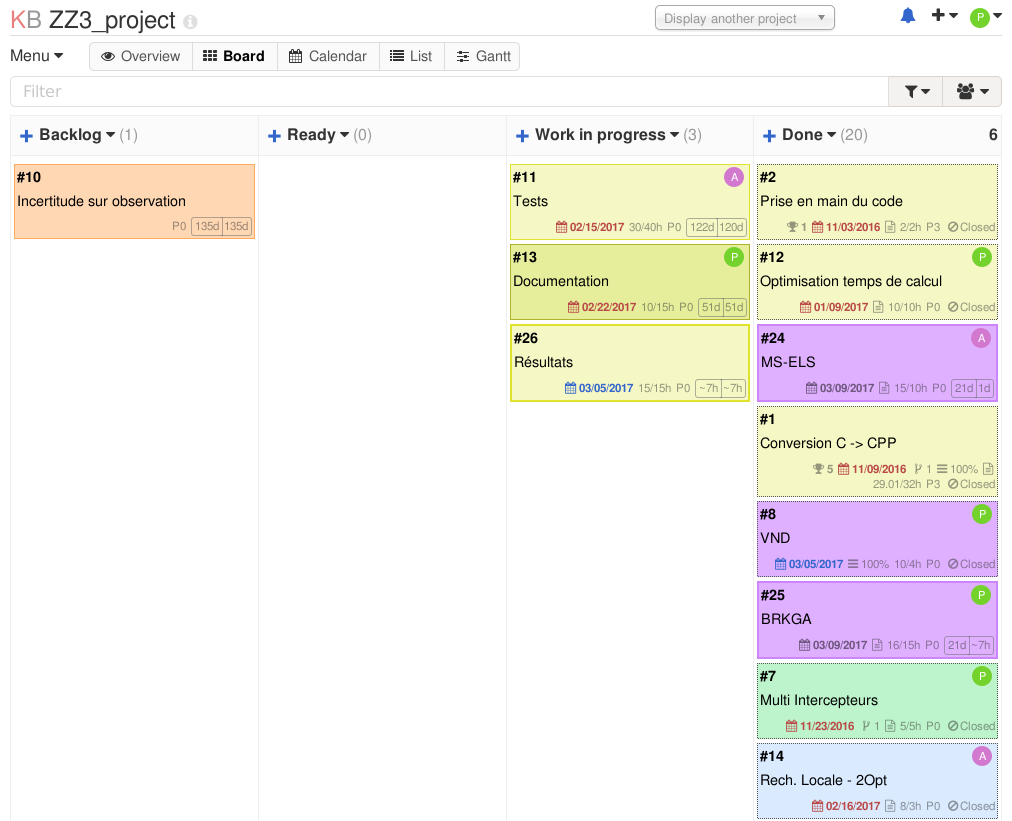
\includegraphics[width=\linewidth]{dashboard}
			\caption{Dashboard de gestion de projet de type Kanban}
			\label{fig:dashboard}
		\end{figure}
